\documentclass[aspectratio=169, table]{beamer}

\usepackage{colortbl}
\usepackage{xcolor}
\usepackage{listings}
\usepackage{xcolor}
\usepackage{pgfplots}
\usepgfplotslibrary{polar}
\usepackage{tikz}
\usetikzlibrary{shapes.geometric, 
	positioning, shapes, shapes.multipart, backgrounds, arrows.meta, calc, fit, trees}

\usetheme{Pradita}



\lstdefinelanguage{bash} {
	keywords={},
	basicstyle=\ttfamily\scriptsize,
	keywordstyle=\color{blue}\bfseries,
	ndkeywords={iex},
	ndkeywordstyle=\color{purple}\bfseries,
	sensitive=true,
	commentstyle=\color{gray},
	stringstyle=\color{red},
	numbers=left,
	numberstyle=\tiny\color{gray},
	breaklines=true,
	frame=lines,
	backgroundcolor=\color{lightgray!10},
	tabsize=2,
	comment=[l]{\#},
	morecomment=[s]{/*}{*/},
	commentstyle=\color{gray}\ttfamily,
	stringstyle=\color{purple}\ttfamily,
	showstringspaces=false,
	captionpos=b
}

% Define Python language style for listings
\lstdefinestyle{PythonStyle}{
    language=Python,
    basicstyle=\ttfamily\footnotesize,
    keywordstyle=\color{blue}\bfseries,
    commentstyle=\color{gray}\itshape,
    stringstyle=\color{red},
    showstringspaces=false,
    breaklines=true,
    frame=lines,
    numbers=left,
    numberstyle=\tiny\color{gray},
    backgroundcolor=\color{lightgray!10},
    tabsize=4,
    captionpos=b
}


\subtitle{IT30213 - Advanced Software Engineering \& DevOps}
\title{\Huge Infratructure as Code \\\vspace{8pt}	
	(IaC)\vspace{5pt}}
%\date[Serial]{Penggunaan Large Language Model untuk Pengajaran}
\author{\textbf{Alfa Yohannis}}
\begin{document}
	
%	\frame{\titlepage}
	

	\begin{frame}[fragile]
		\frametitle{Contents}
		\vspace{20pt}
		\begin{columns}[t]
			\column{0.5\textwidth}
			\tableofcontents[sections={1-5}]
			
			\column{0.5\textwidth}
			\tableofcontents[sections={6-20}]
		\end{columns}
	\end{frame}
	
	\begin{frame}{\hfill}
		\centering
		\Huge{\textbf{How to automate the deployment of our software infrastructure in different environments?}}
	\end{frame}
	

\section{Pendahuluan}

\begin{frame}{Pendahuluan}
	\vspace{6pt}
	\begin{itemize}
		\item Arsitektur modern bersifat \textbf{terdistribusi}: API, worker, queue, storage, gateway, observability.
		\item Pengelolaan manual (network, port, credential) meningkatkan risiko \textbf{inkonsistensi} dan kesalahan.
		\item Multi-environment (dev, staging, production) memerlukan pendekatan yang \textbf{sistematis dan reproducible}.
		\item Pendekatan deklaratif melalui IaC mendeskripsikan \textit{desired state}; engine memastikan kondisi aktual sesuai.
		\item Studi kasus: TTS stack (Redis, MinIO, FastAPI API, Web, Worker, Nginx).
		\item Tujuan: konsistensi environment, provisioning otomatis, skalabilitas terkontrol, reproducibility eksperimen, dan audit perubahan infrastruktur.
	\end{itemize}
\end{frame}


\section{Apa itu Infrastructure as Code (IaC)?}

\begin{frame}{Apa itu Infrastructure as Code (IaC)?}
	\vspace{6pt}
	\begin{itemize}
		\item Infrastructure as Code (IaC) adalah pendekatan untuk \textbf{mendefinisikan dan mengelola infrastruktur melalui kode}, bukan konfigurasi manual.
		\item Infrastruktur menjadi bagian dari siklus hidup perangkat lunak: dapat ditulis, direview, diuji, dan dikelola seperti source code.
		\item IaC bersifat \textbf{deklaratif}: kita mendeskripsikan \textit{desired state}, bukan langkah prosedural.
		\item Karakter utama: \textbf{idempotent} (eksekusi berulang tidak mengubah hasil), \textbf{reproducible} (environment dapat dibangun ulang identik), dan terversi melalui Git.
		\item Komponen penting: \textbf{resource definition}, \textbf{dependency graph otomatis}, dan \textbf{state management}.
	\end{itemize}
\end{frame}

\section{Mengapa IaC Diperlukan?}

\begin{frame}{Mengapa IaC Diperlukan?}
	\vspace{6pt}
	\begin{itemize}
		\item Arsitektur modern (microservices, container, cloud) membuat konfigurasi manual menjadi \textbf{tidak efisien dan berisiko}.
		\item Masalah tradisional: \textbf{human error}, inkonsistensi server, environment drift, dan tidak adanya \textit{single source of truth}.
		\item Perubahan infrastruktur sulit diaudit dan sering tidak terdokumentasi dengan baik.
		\item IaC menjadikan infrastruktur sebagai \textbf{artefak kode} yang terversi, dapat direview, dan memiliki riwayat perubahan.
		\item Keuntungan: konsistensi antar environment, provisioning otomatis, diff sebelum perubahan, dan kolaborasi berbasis Git.
		\item Terintegrasi dengan CI/CD untuk provisioning dinamis dan reproducible testing.
	\end{itemize}
\end{frame}

\section{Apa itu Terraform?}

\begin{frame}{Apa itu Terraform?}
	\vspace{6pt}
	\begin{itemize}
		\item Terraform adalah alat \textbf{Infrastructure as Code (IaC)} deklaratif berbasis \textbf{HCL}.
		\item Infrastruktur didefinisikan dalam file \texttt{.tf} sebagai \textit{desired state}.
		\item Alur kerja utama: \texttt{init} → \texttt{plan} (lihat diff) → \texttt{apply} (eksekusi).
		\item Konsep kunci: \textbf{provider} (Docker, AWS, dll.), \textbf{resource}, \textbf{module}, \textbf{variables}, \textbf{outputs}.
		\item Menggunakan \textbf{state file} untuk menghitung perubahan dan mendeteksi drift.
		\item Mendukung reproducibility melalui \texttt{destroy} dan \texttt{apply}.
		\item Cocok untuk multi-environment (dev, staging, production) secara konsisten dan terversi.
	\end{itemize}
\end{frame}

\section{Apa yang Membuat Terraform Berbeda dari Docker Compose?}

\begin{frame}{Terraform vs Docker Compose}
	\vspace{4pt}
	\begin{columns}[T]
		\column{0.5\textwidth}
		\textbf{Docker Compose}
		\begin{itemize}
			\item Fokus pada \textbf{orkestrasi container} di satu host.
			\item Mendefinisikan service, network, dan volume pada Docker Engine.
			\item Tidak memiliki \textbf{state global} atau drift detection formal.
			\item Multi-environment biasanya via override file.
			\item Cocok untuk development, prototyping, dan single-host deployment.
		\end{itemize}

		\column{0.5\textwidth}
		\textbf{Terraform}
		\begin{itemize}
			\item Fokus pada \textbf{provisioning infrastruktur} secara deklaratif (IaC).
			\item Mengelola VM, network, storage, IAM, LB, cluster, dll.
			\item Memiliki \textbf{state file} dan diff melalui \texttt{plan}.
			\item Mendukung modularisasi dan multi-environment via variabel.
			\item Cocok untuk production-grade dan arsitektur terdistribusi.
		\end{itemize}
	\end{columns}
\end{frame}


\section{Contoh Studi Kasus}

	\begin{frame}{\hfill}
		\centering
		\Huge{\textbf{Contoh Studi Kasus}}
	\end{frame}


\begin{frame}{Arsitektur Sistem TTS (Studi Kasus)}
	\vspace{20pt}
	\centering
	\scalebox{0.8}{
	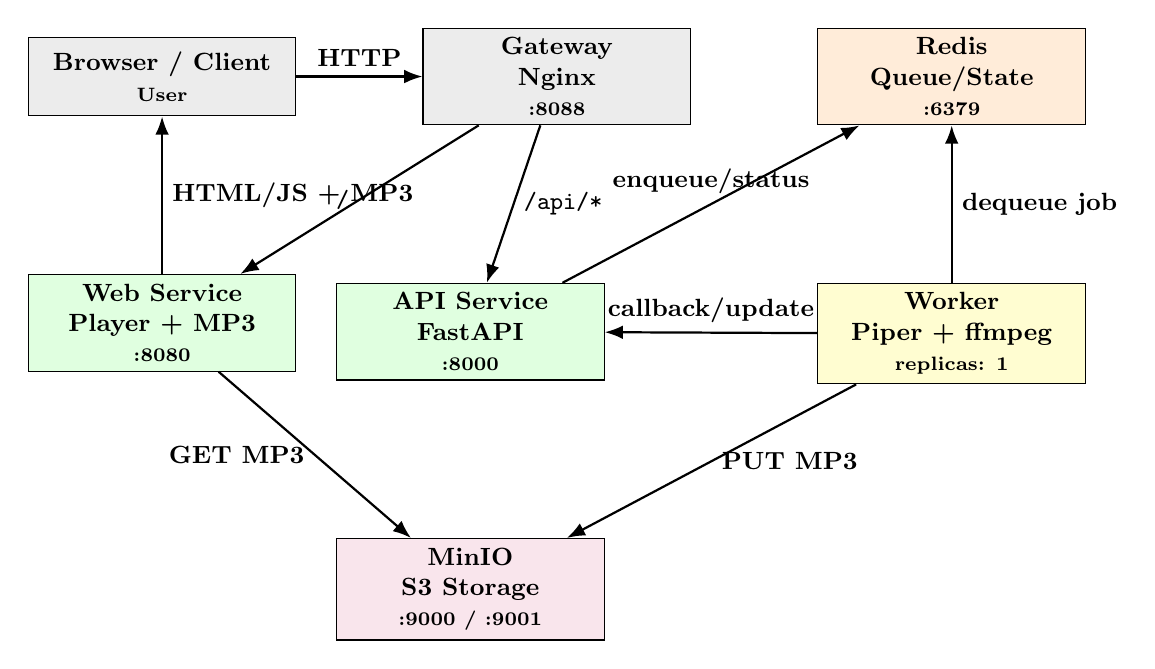
\begin{tikzpicture}[
	  font=\small\bfseries,
	  node distance=20mm and 16mm,
	  box/.style={
	    draw,
	    align=center,
	    minimum width=34mm,
	    minimum height=10mm,
	    fill=blue!10
	  },
	  storebox/.style={box,fill=purple!10},
	  brokerbox/.style={box,fill=orange!15},
	  apiwebbox/.style={box,fill=green!12},
	  gatewaybox/.style={box,fill=gray!15},
	  workerbox/.style={box,fill=yellow!18},
	  annot/.style={font=\scriptsize\itshape, text=black!70},
	  arrow/.style={-Latex,thick}
	]

	% --- Row 1 (top) ---
	\node[gatewaybox] (client) {Browser / Client\\{\scriptsize User}};
	\node[gatewaybox, right=of client] (gateway) {Gateway\\Nginx\\{\scriptsize :8088}};
	\node[brokerbox, right=of gateway] (redis) {Redis\\Queue/State\\{\scriptsize :6379}};

	% --- Row 2 (middle) ---
	\node[apiwebbox, below=of client] (web) {Web Service\\Player + MP3\\{\scriptsize :8080}};
	\node[apiwebbox, below=of gateway, xshift=-11mm] (api) {API Service\\FastAPI\\{\scriptsize :8000}};
	\node[workerbox, below=of redis] (worker) {Worker\\Piper + ffmpeg\\{\scriptsize replicas: 1}};

	% --- Row 3 (bottom) ---
	\node[storebox, below=of api] (minio) {MinIO\\S3 Storage\\{\scriptsize :9000 / :9001}};

	% --- Flows ---
	\draw[arrow] (client) -- node[above]{HTTP} (gateway);
	\draw[arrow] (gateway) -- node[left]{\texttt{/}} (web);
	\draw[arrow] (gateway) -- node[right]{\texttt{/api/*}} (api);
	\draw[arrow] (api) -- node[above]{enqueue/status} (redis);
	\draw[arrow] (worker) -- node[right]{dequeue job} (redis);
	\draw[arrow] (worker) -- node[above]{callback/update} (api);
	\draw[arrow] (worker) -- node[right]{PUT MP3} (minio);
	\draw[arrow] (web) -- node[left]{GET MP3} (minio);
	\draw[arrow] (web) -- node[right]{HTML/JS + MP3} (client);

	\end{tikzpicture}
	}
\end{frame}

\subsection{Workflow}

\begin{frame}{Workflow Terraform Multi-Environment}
	\vspace{15pt}
	\centering
	\scalebox{0.65}{
	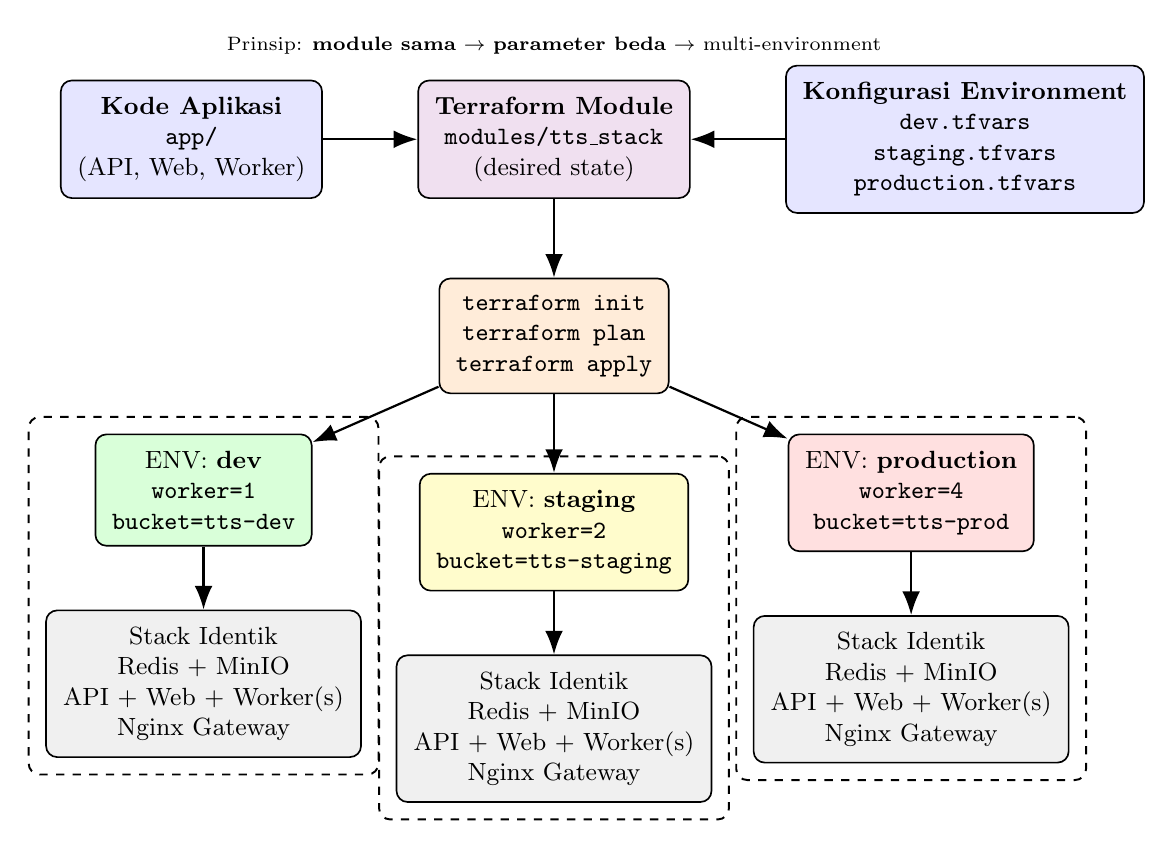
\begin{tikzpicture}[
	  transform shape,
	  font=\small,
	  node distance=10mm and 12mm,
	  box/.style={draw, rounded corners, align=center, inner sep=6pt, line width=0.6pt},
	  inputbox/.style={box, fill=blue!10},
	  modulebox/.style={box, fill=violet!12},
	  planbox/.style={box, fill=orange!15},
	  envdev/.style={box, fill=green!15},
	  envstg/.style={box, fill=yellow!20},
	  envprod/.style={box, fill=red!12},
	  stackbox/.style={box, fill=gray!12},
	  grp/.style={draw, rounded corners, dashed, inner sep=6pt, line width=0.7pt},
	  arr/.style={-{Latex[length=3mm]}, thick},
	  note/.style={align=left, font=\scriptsize}
	]

	\node[inputbox] (code) {\textbf{Kode Aplikasi}\\\texttt{app/}\\(API, Web, Worker)};
	\node[modulebox, right=of code] (module) {\textbf{Terraform Module}\\\texttt{modules/tts\_stack}\\(desired state)};
	\node[inputbox, right=of module] (tfvars) {\textbf{Konfigurasi Environment}\\\texttt{dev.tfvars}\\\texttt{staging.tfvars}\\\texttt{production.tfvars}};

	\node[planbox, below=of module] (plan) {\texttt{terraform init}\\\texttt{terraform plan}\\\texttt{terraform apply}};

	\draw[arr] (code) -- (module);
	\draw[arr] (tfvars) -- (module);
	\draw[arr] (module) -- (plan);

	\node[envdev, below left=5mm and 16mm of plan] (dev) {ENV: \textbf{dev}\\
	\texttt{worker=1}\\
	\texttt{bucket=tts-dev}};
	\node[envstg, below=of plan] (stg) {ENV: \textbf{staging}\\
	\texttt{worker=2}\\
	\texttt{bucket=tts-staging}};
	\node[envprod, below right=5mm and 15mm of plan] (prod) {ENV: \textbf{production}\\
	\texttt{worker=4}\\
	\texttt{bucket=tts-prod}};

	\draw[arr] (plan) -- (dev);
	\draw[arr] (plan) -- (stg);
	\draw[arr] (plan) -- (prod);

	\node[stackbox, below=8mm of dev,  minimum width=40mm] (devstack)
	{Stack Identik\\Redis + MinIO\\API + Web + Worker(s)\\Nginx Gateway};
	\node[stackbox, below=8mm of stg,  minimum width=40mm] (stgstack)
	{Stack Identik\\Redis + MinIO\\API + Web + Worker(s)\\Nginx Gateway};
	\node[stackbox, below=8mm of prod, minimum width=40mm] (prdstack)
	{Stack Identik\\Redis + MinIO\\API + Web + Worker(s)\\Nginx Gateway};

	\node[note, above=2mm of module] (legend)
	{Prinsip: \textbf{module sama} $\rightarrow$ \textbf{parameter beda} $\rightarrow$ multi-environment};

	\draw[arr] (dev) -- (devstack);
	\draw[arr] (stg) -- (stgstack);
	\draw[arr] (prod) -- (prdstack);

	\node[grp, fit=(dev)(devstack)] {};
	\node[grp, fit=(stg)(stgstack)] {};
	\node[grp, fit=(prod)(prdstack)] {};

	\end{tikzpicture}
	}
\end{frame}


\begin{frame}[fragile]{Struktur Proyek Terraform (TTS Stack)}
\vspace{10pt}
\begin{columns}[T]

% ================= LEFT COLUMN =================
\column{0.52\textwidth}
\textbf{Application \& Compose}
\begin{lstlisting}[language=bash]
app/
|- gateway
|  |- nginx.conf
|- models
|  |- en_GB-alan-medium.onnx
|- services
|  |- api
|  |  |- api.py
|  |  |- Dockerfile
|  |- web
|  |  |- web.py
|  |- worker
|     |- worker.py
|- tests
|  |- ...
compose/
|- docker-compose.yml
\end{lstlisting}

% ================= RIGHT COLUMN =================
\column{0.48\textwidth}
\textbf{IaC (Terraform)}
\begin{lstlisting}[language=bash]
iac/
|- terraform
   |- dev
   |  |- main.tf
   |  |- dev.tfvars
   |- staging
   |  |- main.tf
   |  |- staging.tfvars
   |- prod
   |  |- main.tf
   |  |- production.tfvars
   |- modules
      |- tts_stack
         |- main.tf
         |- variables.tf
         |- outputs.tf
\end{lstlisting}

\end{columns}
\end{frame}

\begin{frame}{Struktur Modul dan per Environment}
\vspace{10pt}
\begin{itemize}
    \item \textbf{modules/tts\_stack}: enkapsulasi seluruh resource Docker untuk satu environment.
    \begin{itemize}
        \item \texttt{variables.tf} → kontrak input (env, ports, worker\_replicas, mount\_models).
        \item \texttt{main.tf} → implementasi resource (network, volume, image, container).
        \item \texttt{outputs.tf} → endpoint layanan setelah \texttt{apply}.
    \end{itemize}
    \item Prefix berbasis \texttt{env} (\texttt{tts-dev-*}, \texttt{tts-staging-*}, \texttt{tts-production-*})
          mencegah konflik saat multi-environment berjalan di satu host.
    \item \textbf{Root module} (dev/staging/prod) hanya:
    \begin{itemize}
        \item Memanggil modul yang sama.
        \item Mengisi variabel via \texttt{*.tfvars}.
        \item Mengatur perbedaan port, bucket, token, dan skala worker.
    \end{itemize}
    \item Dev → default \& ringan;  
          Staging → port digeser + 2 worker;  
          Prod → port dedicated + 4 worker + variabel sensitif.
\end{itemize}
\end{frame}


\begin{frame}{Reproducibility dan Skalabilitas}
\vspace{10pt}
\begin{itemize}
    \item Terraform menjadikan infrastruktur sebagai \textbf{desired state deklaratif}, bukan konfigurasi ad-hoc.
    
    \item \textbf{Environment parity}: modul sama digunakan ulang untuk dev, staging, production; 
          perbedaan hanya pada variabel (port, replika, bucket, token).

    \item \textbf{Provisioning terkontrol}: 
          \texttt{init → plan → apply} menampilkan diff sebelum perubahan dieksekusi.

    \item \textbf{Skalabilitas horizontal}: 
          scaling worker cukup mengubah \texttt{worker\_replicas}; 
          Terraform menambah/mengurangi container sesuai state.

    \item \textbf{Kontrol perubahan terstruktur}: 
          state file + version control memungkinkan audit, review, dan rollback.

    \item \textbf{Reproducibility}: 
          environment dapat \texttt{destroy} dan \texttt{apply} ulang secara identik,
          mendukung eksperimen performa dan integrasi CI/CD.
\end{itemize}
\end{frame}


\begin{frame}{Kesimpulan}
	\vspace{10pt}
	\begin{itemize}
		\item \textbf{Infrastructure as Code (IaC)} menjadikan infrastruktur sebagai artefak deklaratif, terversi, dan dapat diaudit.
		\item Mengurangi \textit{environment drift}, inkonsistensi konfigurasi, dan praktik manual yang sulit direproduksi.
		\item Mendukung \textbf{environment parity} antar \texttt{dev}, \texttt{staging}, dan \texttt{production}.
		\item \textbf{Terraform} menyediakan provider, resource, module, variable, output, dan state untuk provisioning terstruktur.
		\item Kombinasi \texttt{plan}/\texttt{apply} + state file memungkinkan diff, drift detection, dan kontrol perubahan.
		\item \textbf{Docker Compose} tetap relevan untuk prototyping lokal; Terraform membawa arsitektur menuju reproducibility dan production-ready.
		\item Keduanya saling melengkapi dalam evolusi sistem dari development ke deployment terkontrol.
	\end{itemize}
\end{frame}

\end{document}
